\graphicspath{{../imgs/}}

\begin{figure}[h!]
    \centering
    \begin{minipage}{0.48\textwidth}
        \centering
        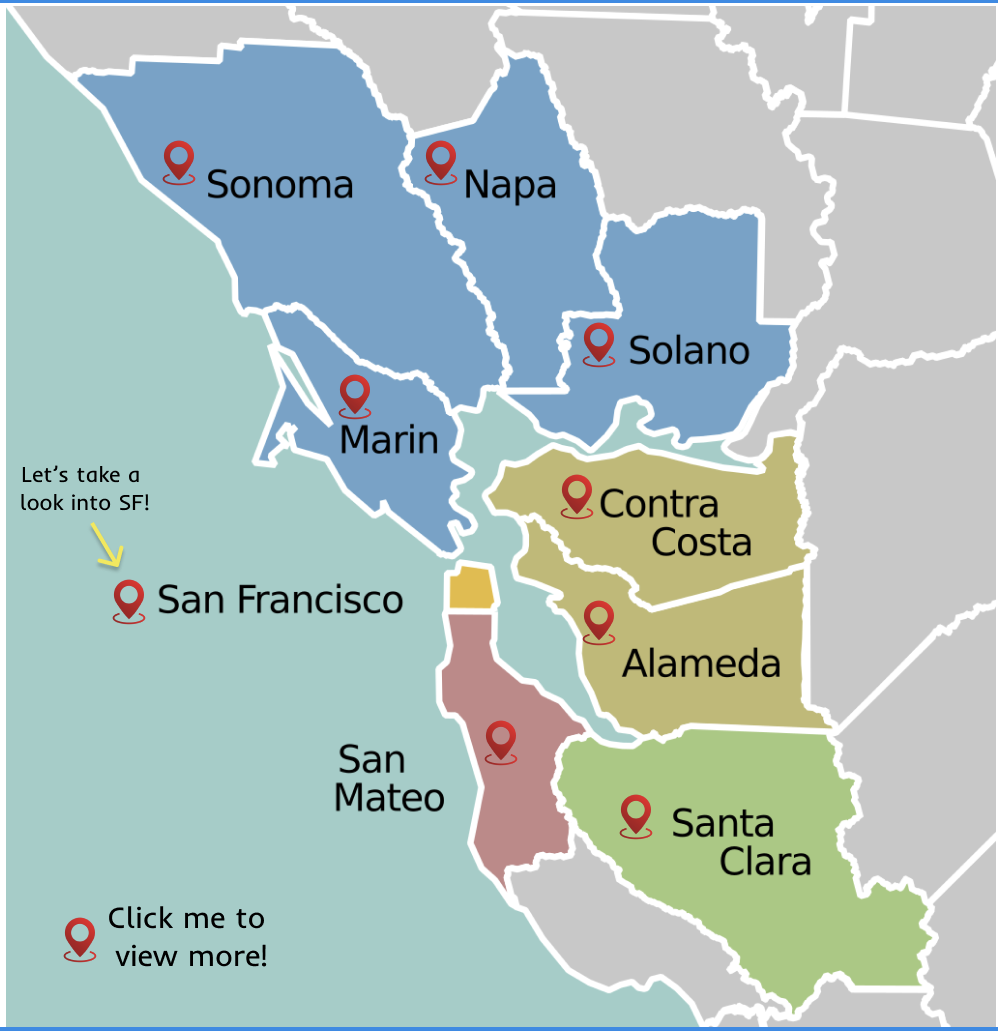
\includegraphics[width=\linewidth]{fig1.png}
        \caption{View of the Bay Area}
        \label{fig:first}
    \end{minipage}\hfill 
    \begin{minipage}{0.48\textwidth}
        \centering
        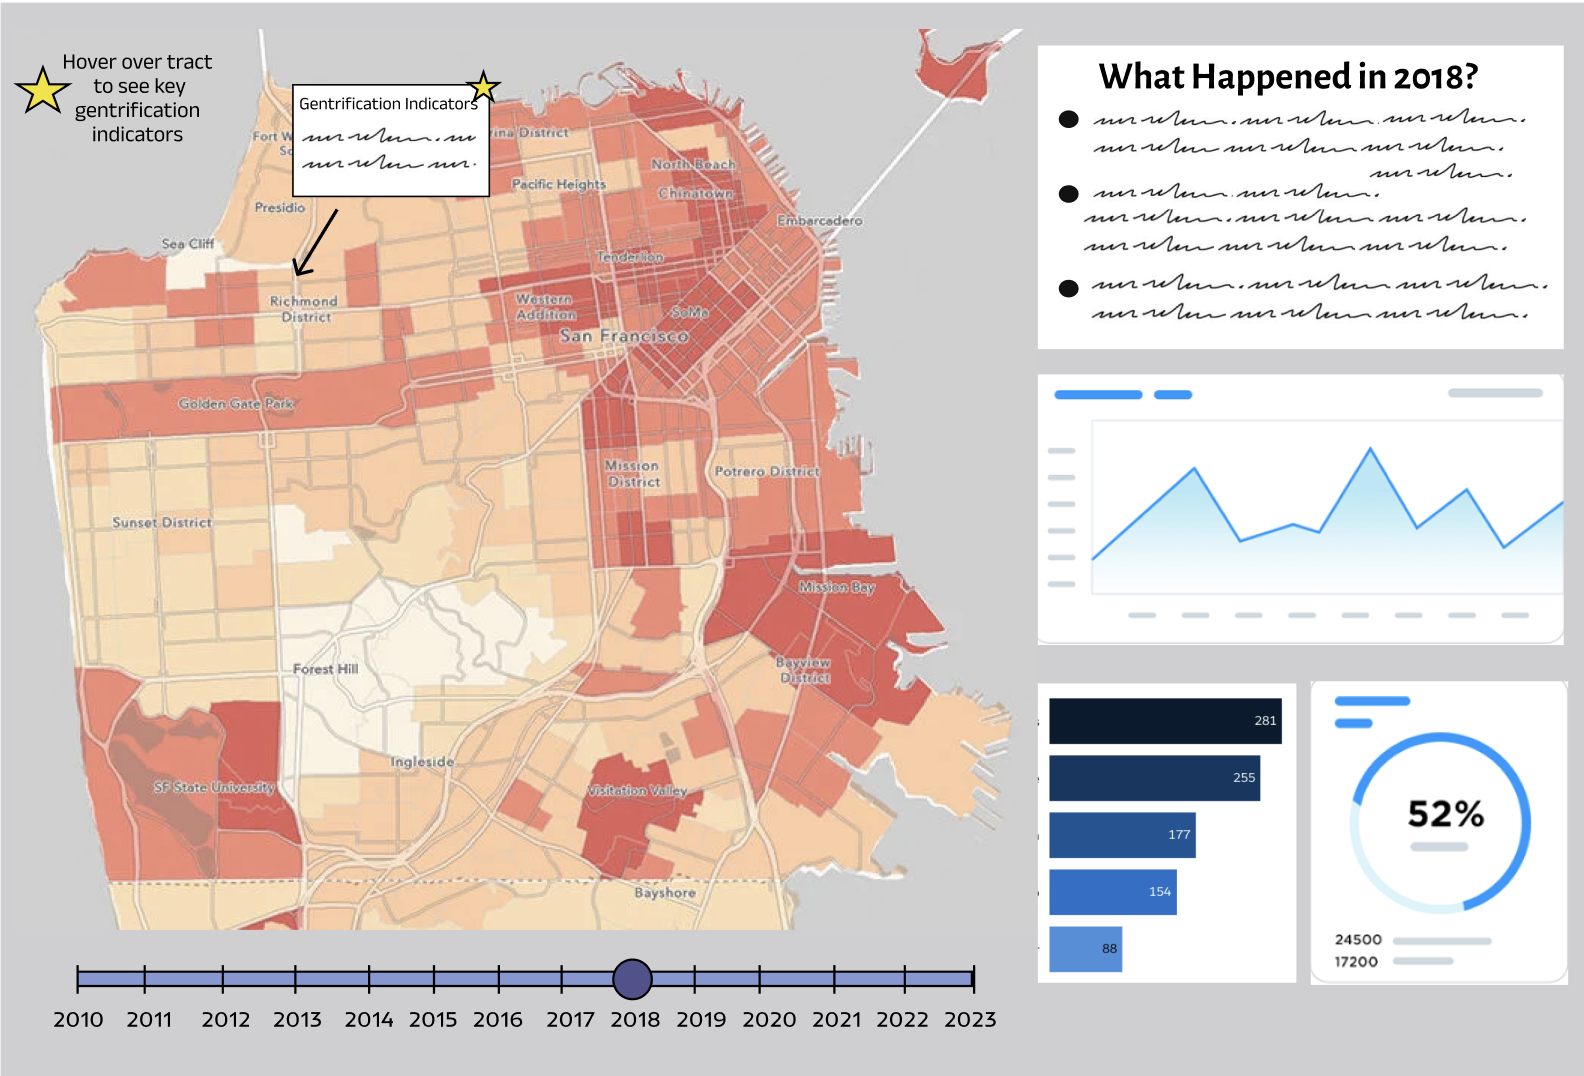
\includegraphics[width=\linewidth]{fig2.png}
        \caption{View of San Francisco County, by census tract}
        \label{fig:second}
    \end{minipage}
    \caption{Drill-Down approach to explore Bay Area counties}
    \label{fig:combined}
\end{figure}